% Template for ICASSP-2021 paper; to be used with:
%          spconf.sty  - ICASSP/ICIP LaTeX style file, and
%          IEEEbib.bst - IEEE bibliography style file.
% --------------------------------------------------------------------------
\documentclass{article}
\usepackage{spconf,amsmath,graphicx,csquotes,siunitx}
%\addbibresource{refs.bib}

% Example definitions.
% --------------------
\def\x{{\mathbf x}}
\def\L{{\cal L}}

% Title.
% ------
\title{Transfer Learning using Musical/Non-Musical Mixtures for Multi-Instrument Classification and Timbre Estimation}
%
% Single address.
% ---------------
\name{Author(s) Name(s)\thanks{Thanks to XYZ agency for funding.}}
\address{Author Affiliation(s)}
%
% For example:
% ------------
%\address{School\\
%	Department\\
%	Address}
%
% Two addresses (uncomment and modify for two-address case).
% ----------------------------------------------------------
%\twoauthors
%  {A. Author-one, B. Author-two\sthanks{Thanks to XYZ agency for funding.}}
%	{School A-B\\
%	Department A-B\\
%	Address A-B}
%  {C. Author-three, D. Author-four\sthanks{The fourth author performed the work
%	while at ...}}
%	{School C-D\\
%	Department C-D\\
%	Address C-D}
%
\begin{document}
%\ninept
%
\maketitle
%
\begin{abstract}
%todo: 100-150 words
We propose a two-stage system for automatic identification of instruments in music recordings, determination of their respective loudness and characterization of the timbre of each instrument. The system consists of a classifier and a set of timbre estimators. The classifier is able to identify 15 classes of instruments from a polyphonic mixture. Subsequently, the respective timbre estimators predict several timbre descriptors and the loudness of each instrument present in the mix. Training of all models is split into two phases: After pre-training with a music tagging dataset, the neural networks are retrained using three multi-track datasets. Therefore, different transfer learning (TL) methods are investigated. Training examples are produced on-the-fly by mixing of single-instrument tracks from the multi-track datasets using two different mixing strategies. Finally, classifier and timbre estimators are evaluated in separate experiments. The classifier shows state-of-the-art F1-scores for classes with sufficient training data. For the timbre estimators we obtained decent performance as well, yet the potential of those models is hard to assess, as there is no ground truth or baseline for this task.
\end{abstract}
%
\begin{keywords}
One, two, three, four, five
\end{keywords}
%
\section{Introduction}
\label{sec:intro}

blabla

\section{Method}
\label{sec:method}
blabla

\subsection{Two-Stage System}
\label{sec:method:system}
The proposed system, as depicted in Fig.~\ref{fig:system}, consists of two parts -- a \textit{classifier} and a set of \textit{timbre estimators}. Both subsystems are fed with four-second chunks of the audio mixture. For more info on how this mixture is created, see Section~\ref{sec:method:dataloading}. For each chunk in a batch, the classifier detects present instruments and instrument families according to the taxonomy presented in Section~\ref{sec:method:data}. Subsequently, a set of timbre estimators -- one for each class -- predict various timbre descriptors and the loudness of all instruments or instrument families in the mix. Bear in mind that every timbre estimator is trained to predict features of only one target instrument or instrument family respectively, hence the need for several of these networks.

The classifier's architecture was adopted from~\cite{won2020evaluation}. The proposed network is very similar to a VGG-Net~\cite{simonyan2014very} commonly used for image classification. A stack of convolutional layers, hereafter referred to as \textit{backbone}, is followed by fully connected layers. Before we continue with the classifier, we should briefly talk about the backbone at this point. In an initial step, the time domain signal is converted to a mel-spectrogram with 128 frequency bins. A window length of 512 and a hop size of 256 are used to compute the spectrogram. After that, seven convolutional blocks try to find patterns in this time-frequency representation. Each block consists of a 2D convolutional layer with a kernel size of $3\times3$ followed by batch normalization, ReLU activation and $2\times2$ max pooling. After seven max pooling layers, the frequency dimension is reduced to one. Finally, 1D max pooling is applied over the time axis to shrink the time dimension to one as well. Since the last convolutional layer has 512 kernels, the resulting output representation of the backbone also has a size of 512. After the backbone extracted suitable features from the mel-spectrograms, subsequent fully connected layers learn non-linear combinations of theses features and finally make a decision whether a certain class is active or not. Between the fully connected layers, batchnorm and dropout are applied. In the last layer of the classifier, a sigmoid activation function maps the model's predictions to values between zero and one, hence the outputs can be interpreted as probabilities.

For the timbre estimators, we reuse the architecture of the classifier. Besides adjusting the size of the output layer, we only have to replace the sigmoid activation function of the last layer with a linear activation function, i.e. no activation function, since we want to predict continuous variables (timbre descriptors).

As timbre descriptors, 12 MFCCs, spectral centroid (SPC), spectral flatness (SPF), and zero-crossing rate (ZCR) are used. All timbre descriptors are computed using \textit{librosa}~\cite{mcfee2015librosa} with a frame size of \SI{64}{\milli\second} -- 2048 samples at a sample rate of \SI{32}{\kilo\hertz} -- and \SI{25}{\percent} overlap. Median and interquartile range are calculated for each descriptor to aggregate all frames into a single dimension, hence we end up with a 30-dimensional timbre representation (2*12 MFCCs + 2 SPC + 2 SPF + 2 ZCR). Since we want our models to predict the loudness as well, the timbre estimators' final output layer comprises 31 neurons. The loudness targets for training are computed using an algorithm~\cite{itu2015recommendation} proposed by the \textit{International Telecommunicaton Union (ITU)}.
\begin{figure}[t]
	\begin{minipage}[b]{1.0\linewidth}
		\centering
		\centerline{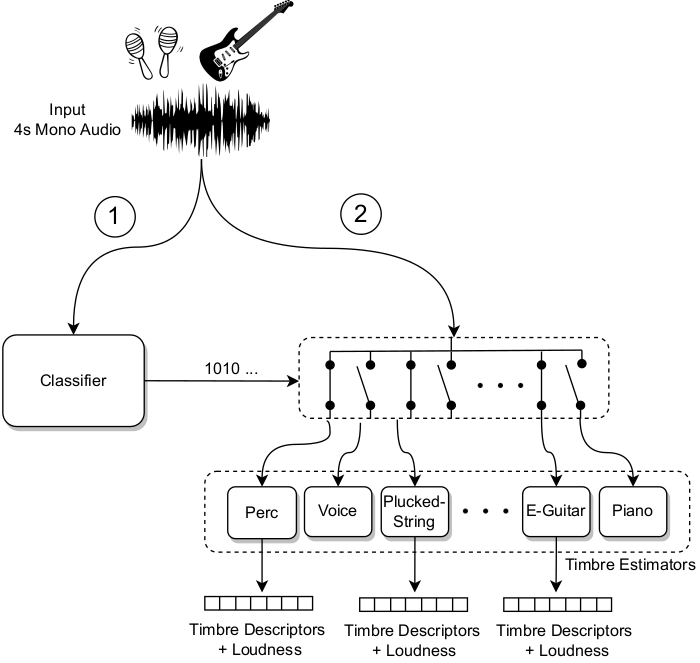
\includegraphics[width=8.25cm,height=7.75cm]{two-stage_system(small).png}}
	\end{minipage}
	\centering
	\caption{Proposed two-stage system. TODO: UMZEICHNEN!!}
	\label{fig:system}
	\vspace*{-0.05cm}	
\end{figure}

\subsection{Data}
\label{sec:method:data}
For TL, a combination of three multi-track datasets is used -- \textit{MedleyDB}~\cite{bittner2014medleydb}, \textit{Mixing Secrets}~\cite{gururani2017mixingsecrets} and \textit{Slakh}~\cite{manilow2019slakh}. Furthermore, \textit{MTG-Jamendo}~\cite{bogdanov2019jamendo}, a large music tagging dataset is utilized for pre-training of all models. This music tagging dataset already comes with a predefined split. However, the multi-track datasets were randomly divided into training, validation and test sets containing \SI{65}{\percent}, \SI{17.5}{\percent} and \SI{17.5}{\percent} of all songs, respectively. We made the decision to split the multi-track datasets at random for the sake of simplicity. Be aware that this practice can potentially lead to overoptimistic results if songs from the same artist or album are contained in multiple splits.

Since the three multi-track datasets used in this work exhibit different class structures, it is necessary to construct a unified instrument taxonomy. Moreover, we want this taxonomy to be hierarchical, hoping that our DNNs can leverage the additional information to learn a broader concept of musical instruments. Similar approaches were already taken several times in the deep learning literature and were successfully implemented for IR applications~\cite{garcia2021leveraging}. As a general rule for training DNNs, a sufficient number of examples for every class is required. In other words, classes with insufficient examples have to be discarded, which basically means that some information gets lost. However, our multi-track datasets are highly imbalanced and for certain instruments only few examples are available. To still utilize these underrepresented classes for training, a two-level hierarchy was defined. It is inspired by the \textit{Hornbostel-Sachs}~\cite{hornbostel1914systematik} system, which classifies musical instruments based on their underlying sound production mechanisms. As the physical principle of an instrument strongly correlates with its sound, such a taxonomy seems appropriate for our use case. The first level of our proposed taxonomy represents eight instrument families: voice, percussion, bowed string, plucked string, woodwind, brass, key and synth. The second level embodies seven specific instruments for which abundant data was available: singer, drums, violin, electric guitar, acoustic guitar, electric bass and piano.

\subsection{Data Loading}
\label{sec:method:dataloading}
Our main data augmentation approach is to create new unique mixtures out of the single-instrument tracks (sources) from the multi-tracks. Therefore, we propose two mixing strategies -- \textit{musical mixing} and \textit{non-musical mixing}. Musical mixing means that only sources from the same song are combined to generate a new mix, whereas non-musical mixing signifies that each source in a mix originates from a different song. The latter, which was successfully used in music source separation~\cite{uhlich2017improving}, obviously results in \enquote{non-musical}, strange sounding mixes, as each instrument plays in a different key and tempo. Nevertheless, the number of training examples can be increased massively by this mixing strategy, which in turn improves generalization. Musical mixing, on the other hand, naturally produces well-sounding results, since all sources originate from the same song and are therefore uniform in tempo and key. In order to investigate the performance of the two proposed mixing strategies, an experiment is conducted in Section~\ref{sec:experiments:classifier:mixing}. Note that for validation and testing, musical mixing was used exclusively, because in real-world recordings, instruments will almost always play in the same key and tempo.

Initially, one of the three multi-track datasets is selected -- each one with the same probability of $1/3$. This step is necessary, because the Slakh dataset is much larger than the other two multi-track datasets. Simply merging them and sampling from the combined dataset would lead to a domination of Slakh samples. However, this should be avoided, because, as already mentioned, the Slakh dataset is synthesized from MIDI files and is therefore quite unrelated to real-world music recordings. In the next step, one of the two proposed mixing strategies is selected. Musical mixing is applied with probability $p_{musical}$ and non-musical mixing is used with probability $1 - p_{musical}$. Then we choose the number of sources $N$ in the mix. As our models should be able to cope with solo-instrument recordings as well, we load single sources ($N=1$) with a certain probability $p_{single-source}$. After that, the following steps are performed $N$ times for the non-musical mixing method: select a song, select a source from this song, select a four-second chunk from this source, apply some digital effects on the audio and add it to the mix. Four audio effects, which have been tried and tested for data augmentation in MIR, are utilized (each with a certain probability): amplitude scaling (gain), three types of filters (high shelf, low shelf and peaking filter), pitch shifting and time stretching. The order of these effects as well as all their parameters are random. Note that, in the musical mixing case, all sources originate from the same song, hence a song is selected only once and not $N$ times (at every loop iteration). Furthermore, the time position of all chunks has to be identical in order to obtain musical sounding results. Finally, pitch shifting and time stretching are omitted for the same reason when musical mixing is applied.

\subsection{Transfer Learning}
\label{sec:method:training}
As our multi-track datasets are relatively small, we decided to adopt a two-step approach, often used by researchers when training data is not sufficient. First of all, the models are pre-trained on \textit{MTG-Jamendo}, a large-scale dataset for music tagging. After that, we experimented with different TL techniques to adapt the pre-trained models to the target tasks. For all TL approaches, we first replaced the fully connected layers of the pre-trained models with new, randomly initialized ones. Furthermore, for the classifier, the size of the output layer was adjusted to 15 to suit the target task of predicting eight instrument families and seven explicit instruments, according to the taxonomy proposed in Section~\ref{sec:method:data}. For the timbre estimators, since we want to predict 31 timbre descriptors, the output layer's size was set to 31. During training with the multi-track data, we either (1) froze the whole backbone network and only retrained the fully connected layers or (2) allowed the backbone to be learnable as well, but with a smaller learning rate than the fully connected layers. As a third method (3) the entire model is trained with the multi-track data from scratch, i.e. not utilizing the pre-trained weights at all. Strictly speaking, method (3) has nothing to do with TL, nevertheless we use it as a reference to show the benefits of methods (1) and (2). The results of these three experiments are discussed in Section~\ref{sec:results:multi-inst_recognition:transfer-learning}. For all experiments, the ADAM optimizer in combination with a stepwise learning rate scheduler was employed. Binary cross-entropy served as a loss function for classification and mean absolute error (MAE) was used for the timbre estimators. Since magnitudes of different timbre descriptors vary greatly, we standardized the targets prior to training.

\section{Experiments}
\label{sec:experiments}
blabla

\subsection{Classifier}
\label{sec:experiments:classifier}
blabla

\subsubsection{Transfer Learning (TL)}
\label{sec:experiments:classifier:tl}
Table~\ref{tab:transfer-learning-experiment} contains the results of the three TL experiments. Unsurprisingly, the performance is worst when no pre-training is exploited and the model is trained from scratch on the multi-track data. Utilizing a pre-trained backbone with frozen parameters significantly increases the performance, indicating that pre-training on a large-scale dataset is beneficial indeed. However, fine-tuning the weights of the backbone to fit the needs of the target task yields additional performance gains. For this reason, the fine-tuning approach is used for all subsequent experiments.
\begin{table}[]
	\centering
	\resizebox{0.4\textwidth}{!}{
	\centering
	\begin{tabular}{c|c|c|c}
		& ROC-AUC & PR-AUC & Test Loss\\ \hline
		From Scratch  & 0.8488 & 0.6812 & 0.4459\\ \hline
		Frozen Backbone  & 0.8908  & 0.7623 & 0.4160\\ \hline
		Fine-tuned & 0.9429  & 0.8334 & 0.3618\\
	\end{tabular}}
	\caption{ROC-AUC, PR-AUC and test loss for different TL approaches.}
	\label{tab:transfer-learning-experiment}
\end{table}

\subsubsection{Mixing Strategy}
\label{sec:experiments:classifier:mixing}
As explained in Section~\ref{sec:method:preprocessing}, our main data augmentation technique is based on mixing of individual sources to create new examples for training. For this reason, the two mixing strategies musical mixing with probability $p_{musical}$ and non-musical mixing with probability $1 - p_{musical}$ are used. To determine the best ratio between these two methods, we experimented with different values for the hyperparameter $p_{musical}$. The experiment was repeated with four distinct seeds and the evaluation metrics were averaged. As depicted in Fig.~\ref{fig:mixing-strategy}, the best performance was obtained for $p_{musical}=0.4$. The result of this investigation suggests, that neither of the two mixing strategies is superior, but rather a combination of both works best. Using only the non-musical mixing approach yields a larger number of training examples. However, the model does not get the chance to learn to identify sources in \enquote{real} music where all instruments play in the same key and tempo. In this case, IR is usually more difficult though, at least for us humans, since masking of individual sources is more pronounced due to synchronous note onsets and overlapping partials. Although overlapping of partials results in consonant sounds, it is substantially harder to distinguish individual sources in this case. On the other hand, if only the musical mixing approach is utilized, fewer training examples can be created, as the number of possible combinations of sources from a single song is limited. Fewer training examples in turn can lead to poorer generalization of the model. We infer from this experiment, that a blend of both mixing strategies yields best results for multi-instrument recognition.
\begin{figure}[t]
	\begin{minipage}[b]{1.0\linewidth}
		\centering
		\centerline{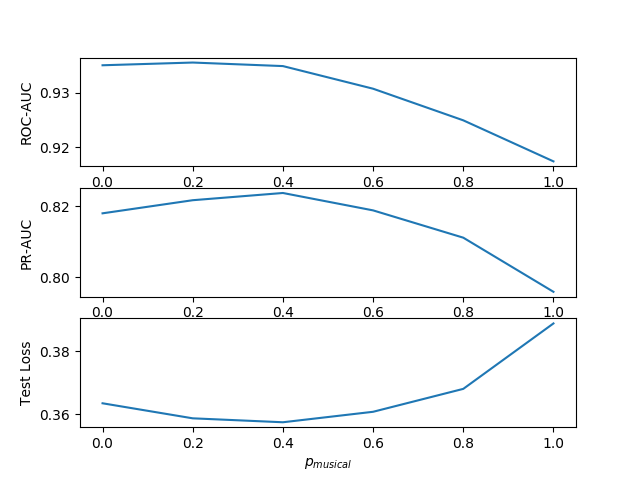
\includegraphics[width=8.5cm,height=7.0cm]{p_mult_songs-experiment.png}}
	\end{minipage}
	\centering
	\caption{ROC-AUC, PR-AUC and test loss for different values of $p_{musical}$.}
	\label{fig:mixing-strategy}
	\vspace*{-0.05cm}	
\end{figure}

\subsubsection{Performance of the Classifier}
\label{sec:experiments:classifier:performance}
Fig.~\ref{fig:f1-scores} shows the performance of our model per class. Unsurprisingly, classes with abundant training data, such as percussion, drums or plucked strings, exhibit the best F1-scores, while identification of instruments or families with insufficient data, like brass, woodwind or violin, does not work well. Note that the F1-score for the brass class is zero because the number of true positives is zero -- no brass instrument was identified correctly. Instead, the model always predicts the absence of the brass family, which is true most of the time, since the brass class is very poorly represented in the data. Apart from that, we obtained state-of-the-art performance for the majority of classes. With F1-scores above \SI{95}{\percent} for some classes, our classifier can easily compete with other recent multi-instrument recognition systems from the literature~\cite{gururani2019attention, seipel2018music, kadandale2018musical}.
\begin{figure}[t]
	\begin{minipage}[b]{1.0\linewidth}
		\centering
		\centerline{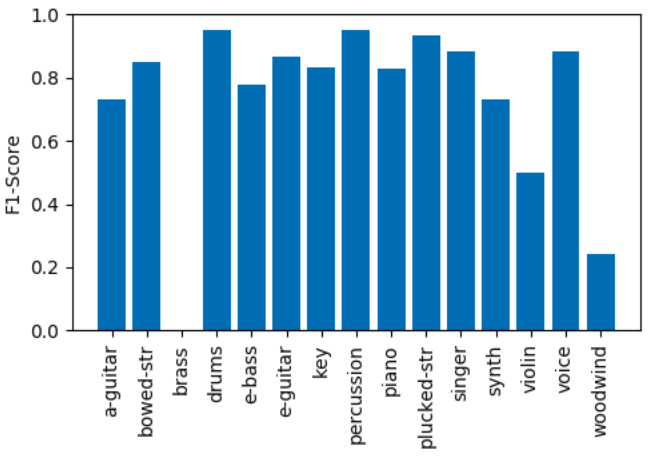
\includegraphics[width=7.5cm,height=4.75cm]{f1-scores.png}}
	\end{minipage}
	\centering
	\caption{Class-wise F1-scores of the classifier.}
	\label{fig:f1-scores}
	\vspace*{-0.05cm}	
\end{figure}

\subsection{Timbre Estimators}
\label{sec:experiments:te}
blabla

\subsubsection{Transfer Learning (TL)}
\label{sec:experiments:te:tl}
The experiment in Section~\ref{sec:experiments:classifier:tl} suggests that utilizing pre-trained convolutional layers and fine-tuning them with the multi-track datasets -- TL method (2) -- yields the best results for our classifier. We repeated the TL experiment with the timbre estimators and found out that TL method (2) works best for the timbre estimators as well.

\subsubsection{Performance of the Timbre Estimators}
\label{sec:experiments:te:performance}
Tables~\ref{tab:feat-pred-mae-fam} and~\ref{tab:feat-pred-mae-class} contain the MAEs we obtained for each model and timbre descriptors. The first thing we note, is that, in general, the performance is better for classes which exhibit smaller within-class variance. However, if the variance within a class is large, the respective timbre estimator has to deal with all those sound variations. For instance, predictions of the synth model are quite poor because the synth class contains all sounds generated by analog or digital sound synthesis according to the taxonomy proposed in Section ???. Since theoretically every conceivable sound can be produced by digital sound synthesis, timbre possibilities within the synth class are endless. Likewise, the performance of the key model is relatively low, since the key class comprises all instruments played with a keyboard -- with the exception of synthesizers. Needless to say, the timbre of instruments within the key class can vary greatly; consider an organ, a piano and an accordion, for example. Furthermore, the relatively poor performance of the percussion and drums models in predicting the zero-crossing rate and the spectral flatness is probably also caused by the high variance within these classes. The bandwidth of percussion instruments is huge, ranging from pitched instruments, such as xylophone or marimba (small zero-crossing rate and spectral flatness), to noise-like instruments, e.g. cymbals or shakers (large zero-crossing rate and spectral flatness). Moreover, the MAEs of the percussion and drums models for spectral centroid prediction is large as well. The reason for that might be similar to the one mentioned above; the high within-class variance of the spectral centroid. The spectrum of a high-pitched triangle and a bass drum could not be more different. Finally, estimation of loudness works best for classes with sufficient training data, such as percussion, plucked strings, voice or drums. With mean errors down to $2.39$ LUFS, the loudness estimation performance in general is more than satisfying.
\begin{table}[]
	\centering
	\resizebox{0.5\textwidth}{!}{
	\centering
	\begin{tabular}{c|c|c|c|c|c|c|c|c}
		& Voice  & Perc   & Pl-Str & Bow-Str& Wood   & Brass  & Key    & Synth \\ \hline
		Loudn    & 3.03   & \textbf{2.74}   & 3.03   & 3.94   & 3.34   & 4.93   & 4.28   & 6.15\\ \hline
		MFCC (Med)& 10.77  & \textbf{7.46}   & 9.94   & 11.85  & 10.86  & 10.98  & 12.03  & 14.24\\ \hline
		MFCC (IQR)& 6.73   & 4.95   & 5.37   & \textbf{4.60}   & 5.62   & 7.07   & 6.05   & 7.13\\ \hline
		SPC (Med)	& 300.8  & 660.3  & \textbf{281.3}  & 481.8  & 401.6  & 427.2  & 293.9  & 498.2\\ \hline
		SPC (IQR) 	& 218.1  & 614.4  & 273.0  & 231.8  & \textbf{209.6}  & 277.6  & 232.6  & 305.4 \\ \hline
		ZCR (Med)  & \textbf{0.0116} & 0.0419 & 0.0117 & 0.0217 & 0.0117 & 0.0234 & 0.0131 & 0.0260\\ \hline
		ZCR (IQR) & 0.0107 & 0.0395 & 0.0105 & 0.0119 & 0.0114 & 0.0125 & \textbf{0.0091} & 0.0096\\ \hline
		SPF (Med)  & 0.0060 & 0.0151 & 0.0003 & 0.0027 & 0.0041 & 0.0327 & \textbf{0.0000} & 0.0009\\ \hline
		SPF (IQR)  & 0.0086 & 0.0197 & 0.0021 & 0.0211 & 0.0181 & 0.0542 & \textbf{0.0006} & 0.0113\\
	\end{tabular}}
	\caption{MAE for every timbre descriptor and instrument family averaged over all test mixes.}
	\label{tab:feat-pred-mae-fam}
\end{table}
\begin{table}[]
	\centering
	\resizebox{0.5\textwidth}{!}{
	\centering
	\begin{tabular}{c|c|c|c|c|c|c|c}
		& Singer & Drums  & Violin & E-Guit & A-Guit & E-Bass & Piano \\ \hline
		Loudn & 3.06   & \textbf{2.39}   & 3.86   & 2.99     & 3.09     & 3.07   & 3.60 \\ \hline
		MFCC (Med)& 10.91  & 7.03   & 11.90  & 9.63     & \textbf{6.89}     & 9.83   & 10.12 \\ \hline
		MFCC (IQR)& 6.80   & 5.11   & 5.00   & 5.30     & \textbf{3.51}     & 5.76   & 5.32\\ \hline
		SPC (Med)	& 300.8  & 804.0  & 470.4  & 183.3    & 313.4    & \textbf{175.9}  & 215.4\\ \hline
		SPC (IQR)	& 220.6  & 805.2  & \textbf{140.4}  & 256.1    & 256.9    & 209.2  & 158.8\\ \hline
		ZCR (Med)& 0.0114 & 0.0382 & 0.0226 & 0.0095   & 0.0134   & \textbf{0.0040} & 0.0102\\ \hline
		ZCR (IQR) & 0.0109 & 0.0453 & 0.0123 & 0.0095   & 0.0100   & \textbf{0.0042} & 0.0068 \\ \hline
		SPF (Med) & 0.0060 & 0.0575 & 0.0007 & 0.0017   & 0.0025   & 0.0019 & \textbf{0.0001} \\ \hline
		SPF (IQR)& 0.0087 & 0.0655 & \textbf{0.0037} & 0.0226   & \textbf{0.0037}   & 0.0112 & 0.0102 \\
	\end{tabular}}
	\caption{MAE for every timbre descriptor and instrument averaged over all test mixes.}
	\label{tab:feat-pred-mae-class}
\end{table}

\section{Conclusion}
\label{sec:conclusion}

blabla ... 






% References should be produced using the bibtex program from suitable
% BiBTeX files (here: strings, refs, manuals). The IEEEbib.bst bibliography
% style file from IEEE produces unsorted bibliography list.
% -------------------------------------------------------------------------
\bibliographystyle{IEEEbib}
\bibliography{refs}
%\printbibliography

\end{document}
